\documentclass[t]{beamer}
\usetheme{hkl}

\title{Linear regression}
	\author{François Briatte \& Ivaylo Petev}
	\date{Week~\#10}

\graphicspath{{images/}}

\begin{document}
    

    % disable footline on title page
    \frame[plain]{
        \titlepage\\[7em]
        \tableofcontents[hideallsubsections]
        }

    
		%
		%

    \section{Multiple linear regression}

	\begin{frame}[c]%{Multiple linear regression}
			
		\begin{center}
			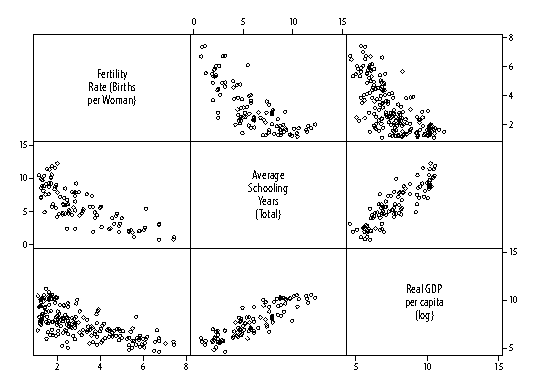
\includegraphics[width=\textwidth]{mreg-gr-mat.pdf}
		\end{center}
				
	\end{frame}
	
	\begin{frame}[c]{Multiple linear regression}
			
		\begin{center}
			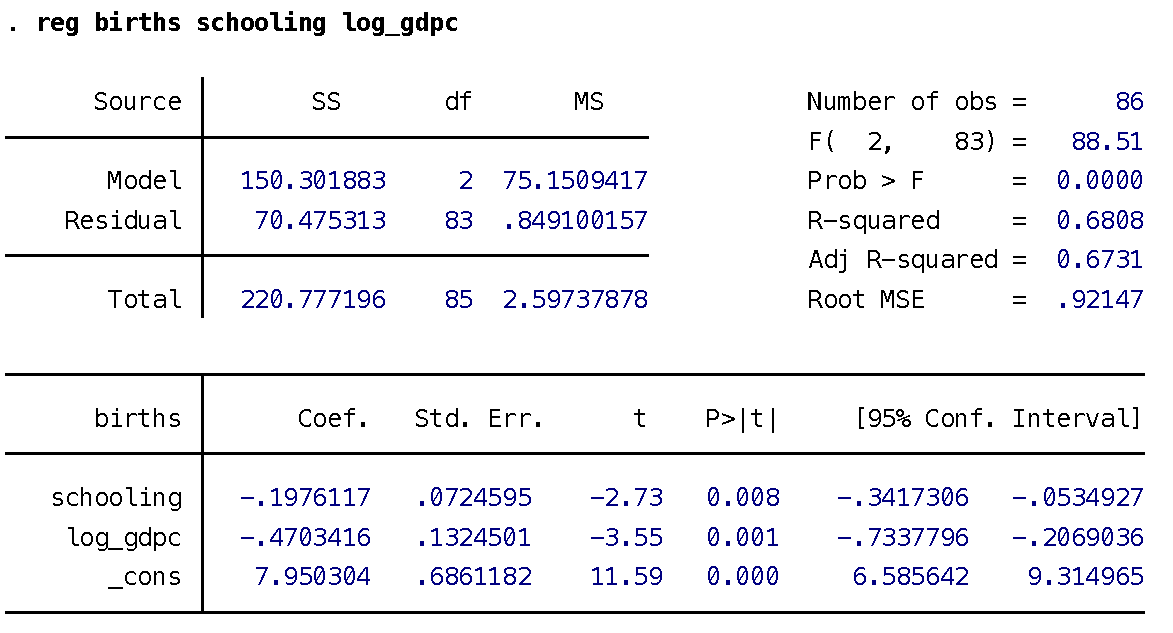
\includegraphics[width=\textwidth]{mreg-output.pdf}
		\end{center}
				
	\end{frame}	
	
	\begin{frame}[c]{Multiple linear regression}
		
		$$Y = \alpha+\beta_1 X_1+\beta_2 X_2+,\ldots,+\beta_k X_k+\epsilon$$
		
		\vfill
		 
		\begin{block}{Partial derivatives}

			Each coefficient is calculated by \red{holding all others constant}.

		\end{block}

		\begin{block}{Least squares}

			The model is still optimized by minimizing the squared error terms.

		\end{block}

		\begin{alertblock}{Sanity check}

			The model is still assuming \emph{linear}, \emph{additive} relationships.

		\end{alertblock}
				
	\end{frame}

	 	%
	%%%%%%%%%%% last page on key regression terms
	%%%%%%
	%%% https://www.princeton.edu/wwac/academic-review/stata/507c/stata_guide.pdf?raw=true
	%%% 
	%%%%%%%%
	%%%%%%%%%

	\begin{frame}[c]{Lin-log coefficients: see \href{http://www.ats.ucla.edu/stat/mult_pkg/faq/general/log_transformed_regression.htm}{UCLA mini-guide}}
	
	\begin{block}{Linear-linear relationships}
		$Y = \beta_0 + \beta_1 X$: an increase of one unit of $X$ is associated with an increase of $\beta_1$ units of $Y$.
	\end{block}
	
	\begin{block}{Log-linear relationships}
		$\red{\ln Y} = \beta_0 + \beta_1 X$: an increase of one unit of $X$ is associated with a $100 \times \beta_1$\% increase in $Y$ (true effect: $Y \times$ \texttt{exp($\beta_1$)}).
	\end{block}

	\begin{block}{Linear-log relationships}
		$Y = \beta_0 + \red{\beta_1 \ln X}$: a 1\% increase in $X$ is associated with a $0.01 \times \beta_1$ unit increase in $Y$ (e.g. $\beta_1 \times$ \texttt{log(1.15)} for +15\% in $X$).
	\end{block}
	
	\begin{block}{Log-log relationships}
		$\red{\ln Y} = \beta_0 + \red{\beta_1 \ln X}$: a 1\% increase in $X$ is associated with a $\beta_1$\%
		increase in $Y$.
	\end{block}
	
	\end{frame}
	
		\section{Standardized coefficients}

	\begin{frame}[t]{\texttt{reg births schooling log\_gdpc\red{, beta}}}

		Each variable can be normalized to fit $\mathcal{D} \sim \mathcal{N}(0,1)$, so that their \red{standardized coefficients} have comparable standard deviation units:
		
		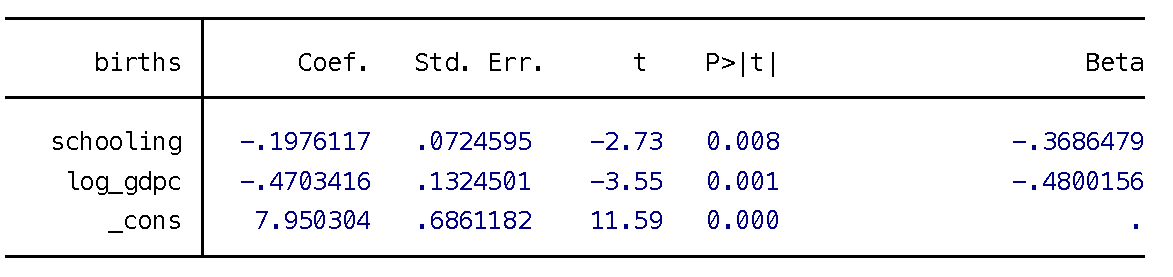
\includegraphics[scale=.45]{mreg-output-beta.pdf}

		\footnotesize{\textit{(identical output for overall model fit omitted)}}
		
		\begin{alertblock}{Sanity check}

			Interpret unstandardized coefficients; use standardization only for model comparisons.

		\end{alertblock}

	\end{frame}

		\section{Regression dummies}
			
	\begin{frame}[t]{\texttt{reg births schooling log\_gdpc \red{i.region}}}

		Categorical variables can be used as \red{dummies}, i.e. binary recodes of each category that are tested against a \red{reference category} to provide regression coefficients for the net effect of each category:\\[.5em]

		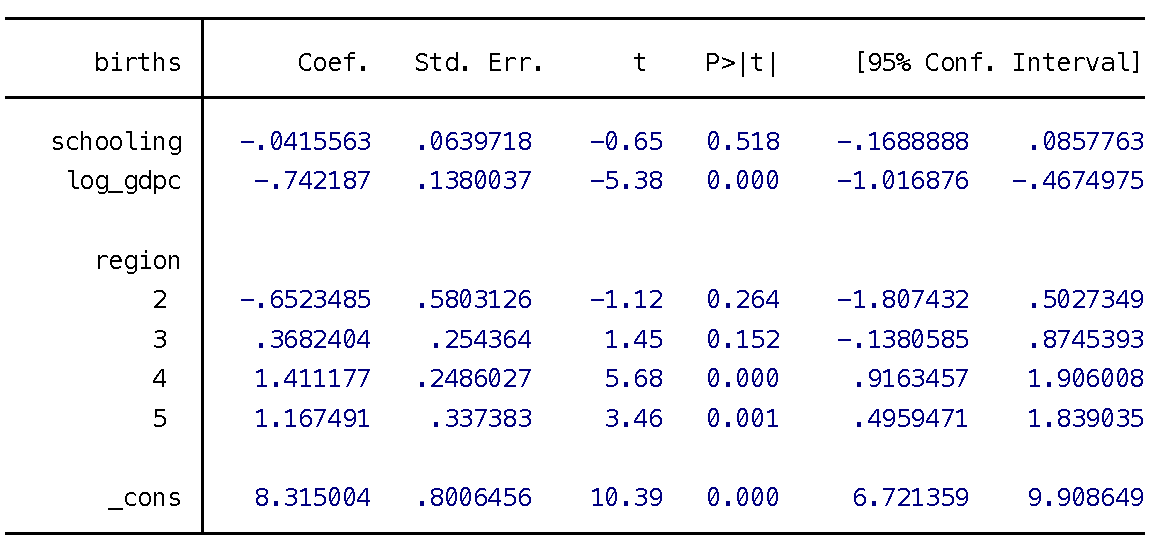
\includegraphics[scale=.45]{mreg-output-dummies.pdf}

		\footnotesize{\textit{(identical output for overall model fit omitted)}}

	\end{frame}

	\section{Regression diagnostics}
	
	\begin{frame}[t]{Regression diagnostics}

		\begin{block}{Residuals}

			\begin{itemize}
				\item \texttt{predict yhat}: fitted values
				\item \texttt{predict r, resid}: residuals
				\item \texttt{predict r, rsta}: standardized residuals		
			\end{itemize}
			
			Use \texttt{rvfplot} for residuals-versus-fitted values plots.

		\end{block}

		\begin{block}{Interaction terms}

			\begin{itemize}
				\item Use \texttt{vif} to detect variables with $VIF > 10$
				\item Use \texttt{c.} and \texttt{\#} for interactions
			\end{itemize}

		\end{block}
		
	\end{frame}

    %
    %

    \begin{frame}[c]{Thanks for your attention}
    
        \begin{alertblock}{Project}
            \begin{itemize}
                \item Name your paper and do-file like \red{Briatte\_Petev\_2}
                \item Make sure to print your paper to a slick \red{PDF}
            \end{itemize}
        \end{alertblock}
        
        \begin{block}{Readings}
            \begin{itemize}
                \item \emph{Stata Guide}, Sec.~10, 11, 13 and 15
            \end{itemize}
        \end{block}
            
        \begin{exampleblock}{Practice}
            \begin{itemize}
                \item Replicate do-file
                \item \red{Use its structure for Draft No.~2}
            \end{itemize}
        \end{exampleblock}
            
    \end{frame}
    
\end{document}
